\subsection{Stepper Motor}


\begin{tabular}{@{}ll}
    \textbf{Type:} & Creality CR - M4 42-34 Motor \\
    \textbf{Voltage:} & Max 1A \\
    \textbf{Current Range:} & Ideally 0.9A - 1.2A (Motor cracking sound below this range) \\
    \textbf{Current Range:} & 0.3A to 2.5A (Source: \url{https://www.youtube.com/watch?v=7spK_BkMJys}) \\
    \textbf{Holding Torque:} & 2.86 kg.cm Type \\
\end{tabular}


\subsection{Stepper Motor Driver}

\textbf{Old Stepper Motor Driver}

\begin{tabular}{@{}ll}
    \textbf{Type:} & A4988 \\
    \textbf{Recommended Current:} & Max 1A \\
    \textbf{Microstepping:} & \\
\end{tabular}

\noindent
\textbf{New Stepper Motor Driver}

\begin{tabular}{@{}ll}
    \textbf{Type:} & TMC2208? \\
\end{tabular}

% 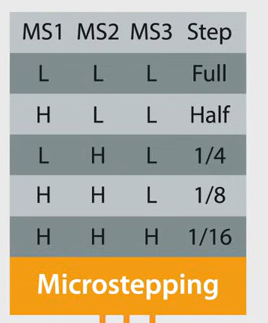
\includegraphics[width=0.7\textwidth]{image.png}

\subsection{Arduino CNC Shield}

\begin{tabular}{@{}ll}
    \textbf{Type:} & Arduino Mega CNC shield: RAMPS 1.4  \\
    \textbf{Url:} & \url{https://www.manomano.fr/p/3d-controleur-dimprimante-ramps-14-mega-shield-pour-arduino-reprap-prusa-mendel-86220892} \\
\end{tabular}

In order to run pn 24 volt, you have to disconnect the board from the ardiono Mega by removing a diode.
This is explained in detail here: \url{https://reprap.org/wiki/RAMPS_24v}.

\subsection{Temperature Sensor}

\textbf{Type:} NTC 10K, B57164 - K103 - K

\textbf{Resistance Values:}
\begin{itemize}
    \item 25$^\circ$C: Approximately 6,000 Ohm
    \item 50$^\circ$C: Approximately 2,000 Ohm (Target: 1,000 Ohm).  A parallel resistor of 2 kOhm is needed.
\end{itemize}

\subsection{Leadscrew, Nut, and Coupler}

\textbf{Nut:} \url{https://www.123-3d.nl/123-3D-Leadscrew-moer-TR8x8-i1560-t9712.html}

\textbf{Coupler:} \url{https://www.123-3d.nl/123-3D-Flexibele-motor-koppeling-5-mm-8-mm-i342-t3045.html}

\textbf{Leadscrew:} \url{https://www.123-3d.nl/123-3D-Leadscrew-TR8x8-8-mm-30-cm-i1558-t9712.html}

\textbf{Heating Wire:} \url{https://www.amazon.com.be/-/en/Meter-Silicone-Rubber-Heating-Electric/dp/B0CD1BSY5F?th=1}